\documentclass[12pt, twoside]{article}
\usepackage[letterpaper, margin=1in, headsep=0.5in]{geometry}
\usepackage[english]{babel}
\usepackage[utf8]{inputenc}
\usepackage{amsmath}
\usepackage{amsfonts}
\usepackage{amssymb}
\usepackage{tikz}
\usetikzlibrary{quotes, angles}
\usepackage{graphicx}
%\usepackage{pgfplots}
%\pgfplotsset{width=10cm,compat=1.9}
%\usepgfplotslibrary{statistics}
%\usepackage{pgfplotstable}
%\usepackage{tkz-fct}
%\usepackage{venndiagram}
\usepackage{multicol}


\usepackage{fancyhdr}
\pagestyle{fancy}
\fancyhf{}
\fancyhead[LE]{\thepage}
\fancyhead[RO]{\thepage \\Name: \hspace{4cm} \,\\}
\fancyhead[LO]{BECA / Dr. Huson / Geometry 10th Grade\\* Unit 9: Congruence transformations \\ 25 February 2020}

\renewcommand{\headrulewidth}{0pt}

\begin{document}
\subsubsection*{9.2b Do Now: Transformations}
  \begin{enumerate}

  \item A transformation is applied to a triangle, $\triangle CAT \rightarrow \triangle C'A'T'$.  Circle True or False to identify each transformation correctly represented below.  \vspace{0.5cm}
    \begin{multicols}{2}
    \begin{itemize}
      \item[T \quad F \quad] Translated six to the left, down zero
      \item[T \quad F \quad] Reflected across the $y$-axis
      \item[T \quad F \quad] $(x,y) \rightarrow (x-6, y+0)$
      \item[T \quad F \quad] Rotated $90^\circ$ counterclockwise around the origin
      \item[T \quad F \quad] A slide six units to the right
    \end{itemize}
    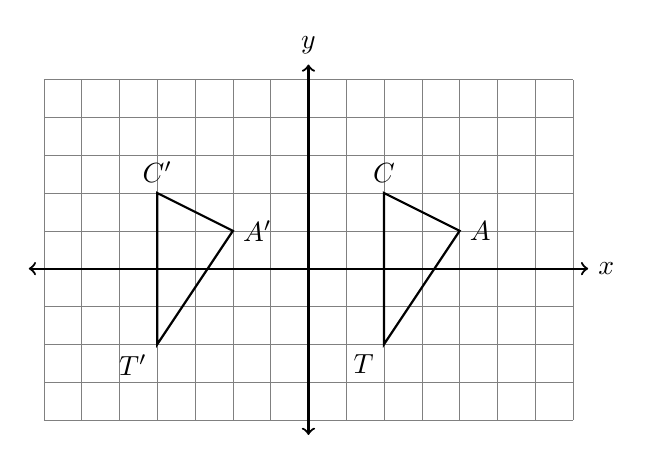
\begin{tikzpicture}[scale=.48]
      \draw [help lines] (-7,-4) grid (7,5);
      \draw [thick, <->] (-7.4,0) -- (7.4,0) node [right] {$x$};
      \draw [thick, <->] (0,-4.4)--(0,5.4) node [above] {$y$};  
      \draw [thick]
      (2,2) node[above] {$C$}--
      (4,1) node[right] {$A$}--
      (2,-2) node[below left] {$T$}--cycle;
      \draw [thick]
      (-4,2) node[above] {$C'$}--
      (-2,1) node[right] {$A'$}--
      (-4,-2) node[below left] {$T'$}--cycle;
    \end{tikzpicture}
  \end{multicols}
  
  \item Determine and state the transformation mapping $\triangle ABC$ onto $\triangle DEF$.
  \begin{flushright}
      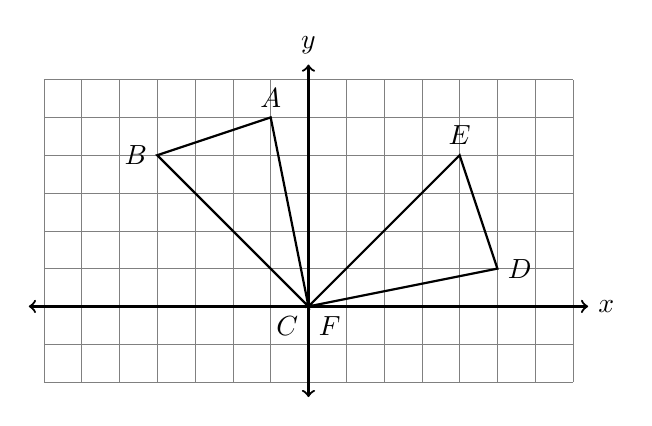
\begin{tikzpicture}[scale=.48]
      \draw [help lines] (-7,-2) grid (7,6);
      \draw [thick, <->] (-7.4,0) -- (7.4,0) node [right] {$x$};
      \draw [thick, <->] (0,-2.4)--(0,6.4) node [above] {$y$};  
      \draw [thick]
        (-1,5) node[above] {$A$}--
        (-4,4) node[left] {$B$}--
        (0,0) node[below left] {$C$}--cycle;
      \draw [thick]
      (5,1) node[right] {$D$}--
      (4,4) node[above] {$E$}--
      (0,0) node[below right] {$F$}--cycle;
    \end{tikzpicture}
  \end{flushright}

  \item Reflect the trapezoid $BECA$ across the $x$-axis. Label the image $B'E'C'A'$.
  \begin{center}
      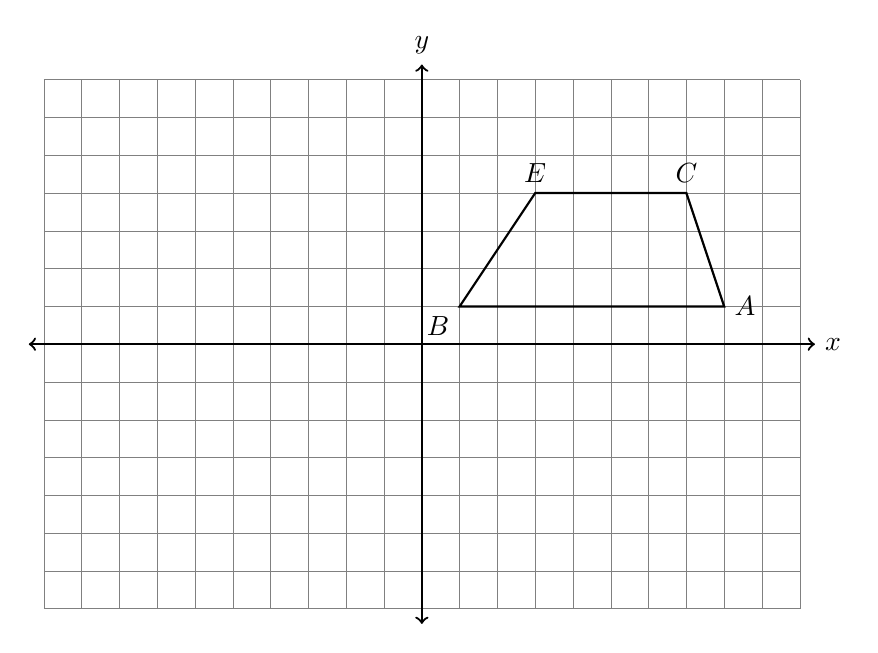
\begin{tikzpicture}[scale=.48]
      \draw [help lines] (-10,-7) grid (10,7);
      \draw [thick, <->] (-10.4,0) -- (10.4,0) node [right] {$x$};
      \draw [thick, <->] (0,-7.4)--(0,7.4) node [above] {$y$};  
      \draw [thick]
        (1,1) node[below left] {$B$}--
        (3,4) node[above] {$E$}--
        (7,4) node[above] {$C$}--
        (8,1) node[right] {$A$}--cycle;  
    \end{tikzpicture}
  \end{center}

\newpage
\subsubsection*{Classwork: Composition of a sequence of transformations}
  \item Two translations have been applied to a triangle in the diagram below, $\triangle ABC \rightarrow \triangle A'B'C' \rightarrow \triangle A''B''C''$. State each translation.
    \begin{center}
        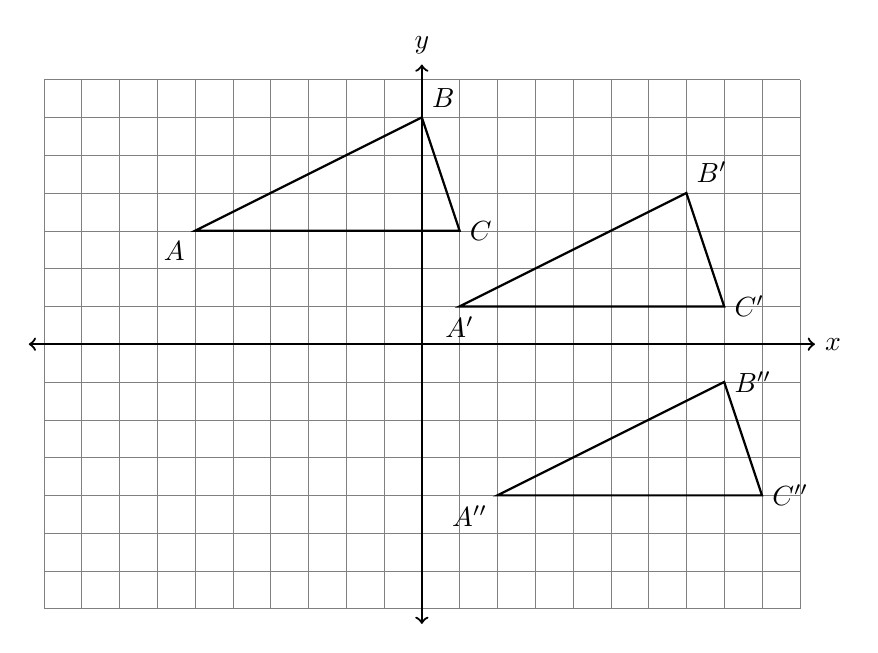
\begin{tikzpicture}[scale=.48]
        \draw [help lines] (-10,-7) grid (10,7);
        \draw [thick, <->] (-10.4,0) -- (10.4,0) node [right] {$x$};
        \draw [thick, <->] (0,-7.4)--(0,7.4) node [above] {$y$};  
        \draw [thick]
          (-6,3) node[below left] {$A$}--
          (0,6) node[above right] {$B$}--
          (1,3) node[right] {$C$}--cycle;
        \draw [thick]
          (1,1) node[below] {$A'$}--
          (7,4) node[above right] {$B'$}--
          (8,1) node[right] {$C'$}--cycle;  
          \draw [thick]
          (2,-4) node[below left] {$A''$}--
          (8,-1) node[right] {$B''$}--
          (9,-4) node[right] {$C''$}--cycle;
      \end{tikzpicture}
    \end{center} \vspace{2cm}
    
  \item The quadrilateral $ROCK$ undergoes two transformations, shown below. Describe the sequence of transformations applied.
  \begin{center}
      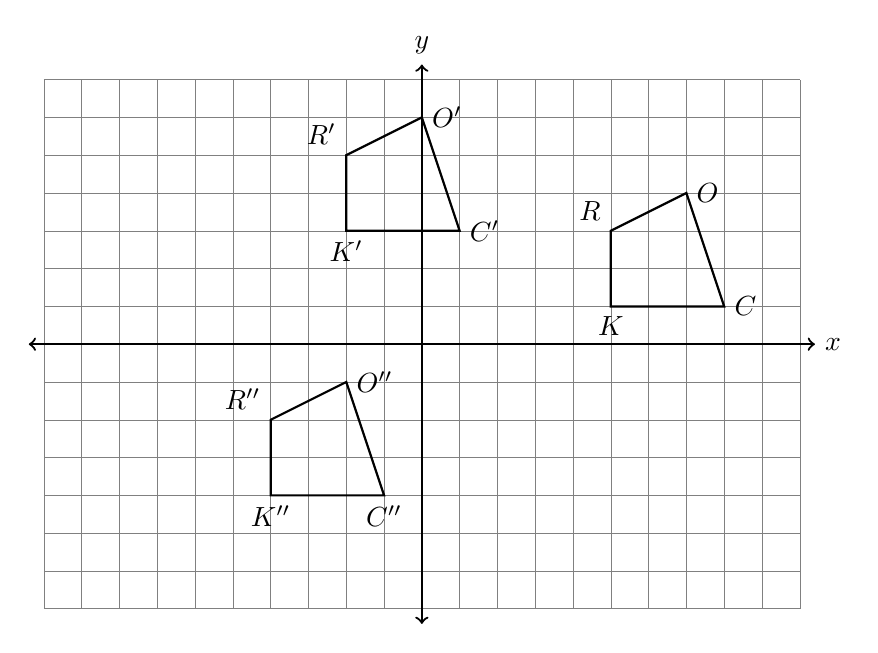
\begin{tikzpicture}[scale=.48]
      \draw [help lines] (-10,-7) grid (10,7);
      \draw [thick, <->] (-10.4,0) -- (10.4,0) node [right] {$x$};
      \draw [thick, <->] (0,-7.4)--(0,7.4) node [above] {$y$};  
      \draw [thick]
        (5,1) node[below] {$K$}--
        (5,3) node[above left] {$R$}--
        (7,4) node[right] {$O$}--
        (8,1) node[right] {$C$}--cycle;
      \draw [thick]
        (-2,3) node[below] {$K'$}--
        (-2,5) node[above left] {$R'$}--
        (0,6) node[right] {$O'$}--
        (1,3) node[right] {$C'$}--cycle;  
      \draw [thick]
      (-4,-4) node[below] {$K''$}--
      (-4,-2) node[above left] {$R''$}--
      (-2,-1) node[right] {$O''$}--
      (-1,-4) node[below] {$C''$}--cycle;
    \end{tikzpicture}
  \end{center}


\end{enumerate}
\end{document}
